\documentclass[11pt]{article}

    \usepackage[breakable]{tcolorbox}
    \usepackage{parskip} % Stop auto-indenting (to mimic markdown behaviour)
    \usepackage{colortbl}
        \usepackage{float}
        \usepackage{rotating}
        \usepackage[table*]{xcolor}
        \usepackage{tabularx}
        \usepackage{siunitx}
        \sisetup{output-exponent-marker=\text{e}}
        \xdefinecolor{gray95}{gray}{0.65}
        \xdefinecolor{gray25}{gray}{0.8}

    % Basic figure setup, for now with no caption control since it's done
    % automatically by Pandoc (which extracts ![](path) syntax from Markdown).
    \usepackage{graphicx}
    % Keep aspect ratio if custom image width or height is specified
    \setkeys{Gin}{keepaspectratio}
    % Maintain compatibility with old templates. Remove in nbconvert 6.0
    \let\Oldincludegraphics\includegraphics
    % Ensure that by default, figures have no caption (until we provide a
    % proper Figure object with a Caption API and a way to capture that
    % in the conversion process - todo).
    \usepackage{caption}
    \DeclareCaptionFormat{nocaption}{}
    \captionsetup{format=nocaption,aboveskip=0pt,belowskip=0pt}

    \usepackage{float}
    \floatplacement{figure}{H} % forces figures to be placed at the correct location
    \usepackage{xcolor} % Allow colors to be defined
    \usepackage{enumerate} % Needed for markdown enumerations to work
    \usepackage{geometry} % Used to adjust the document margins
    \usepackage{amsmath} % Equations
    \usepackage{amssymb} % Equations
    \usepackage{textcomp} % defines textquotesingle
    % Hack from http://tex.stackexchange.com/a/47451/13684:
    \AtBeginDocument{%
        \def\PYZsq{\textquotesingle}% Upright quotes in Pygmentized code
    }
    \usepackage{upquote} % Upright quotes for verbatim code
    \usepackage{eurosym} % defines \euro

    \usepackage{iftex}
    \ifPDFTeX
        \usepackage[T1]{fontenc}
        \IfFileExists{alphabeta.sty}{
              \usepackage{alphabeta}
          }{
              \usepackage[mathletters]{ucs}
              \usepackage[utf8x]{inputenc}
          }
    \else
        \usepackage{fontspec}
        \usepackage{unicode-math}
    \fi

    \usepackage{fancyvrb} % verbatim replacement that allows latex
    \usepackage{grffile} % extends the file name processing of package graphics
                         % to support a larger range
    \makeatletter % fix for old versions of grffile with XeLaTeX
    \@ifpackagelater{grffile}{2019/11/01}
    {
      % Do nothing on new versions
    }
    {
      \def\Gread@@xetex#1{%
        \IfFileExists{"\Gin@base".bb}%
        {\Gread@eps{\Gin@base.bb}}%
        {\Gread@@xetex@aux#1}%
      }
    }
    \makeatother
    \usepackage[Export]{adjustbox} % Used to constrain images to a maximum size
    \adjustboxset{max size={0.9\linewidth}{0.9\paperheight}}

    % The hyperref package gives us a pdf with properly built
    % internal navigation ('pdf bookmarks' for the table of contents,
    % internal cross-reference links, web links for URLs, etc.)
    \usepackage{hyperref}
    % The default LaTeX title has an obnoxious amount of whitespace. By default,
    % titling removes some of it. It also provides customization options.
    \usepackage{titling}
    \usepackage{longtable} % longtable support required by pandoc >1.10
    \usepackage{booktabs}  % table support for pandoc > 1.12.2
    \usepackage{array}     % table support for pandoc >= 2.11.3
    \usepackage{calc}      % table minipage width calculation for pandoc >= 2.11.1
    \usepackage[inline]{enumitem} % IRkernel/repr support (it uses the enumerate* environment)
    \usepackage[normalem]{ulem} % ulem is needed to support strikethroughs (\sout)
                                % normalem makes italics be italics, not underlines
    \usepackage{soul}      % strikethrough (\st) support for pandoc >= 3.0.0
    \usepackage{mathrsfs}
    

    
    % Colors for the hyperref package
    \definecolor{urlcolor}{rgb}{0,.145,.698}
    \definecolor{linkcolor}{rgb}{.71,0.21,0.01}
    \definecolor{citecolor}{rgb}{.12,.54,.11}

    % ANSI colors
    \definecolor{ansi-black}{HTML}{3E424D}
    \definecolor{ansi-black-intense}{HTML}{282C36}
    \definecolor{ansi-red}{HTML}{E75C58}
    \definecolor{ansi-red-intense}{HTML}{B22B31}
    \definecolor{ansi-green}{HTML}{00A250}
    \definecolor{ansi-green-intense}{HTML}{007427}
    \definecolor{ansi-yellow}{HTML}{DDB62B}
    \definecolor{ansi-yellow-intense}{HTML}{B27D12}
    \definecolor{ansi-blue}{HTML}{208FFB}
    \definecolor{ansi-blue-intense}{HTML}{0065CA}
    \definecolor{ansi-magenta}{HTML}{D160C4}
    \definecolor{ansi-magenta-intense}{HTML}{A03196}
    \definecolor{ansi-cyan}{HTML}{60C6C8}
    \definecolor{ansi-cyan-intense}{HTML}{258F8F}
    \definecolor{ansi-white}{HTML}{C5C1B4}
    \definecolor{ansi-white-intense}{HTML}{A1A6B2}
    \definecolor{ansi-default-inverse-fg}{HTML}{FFFFFF}
    \definecolor{ansi-default-inverse-bg}{HTML}{000000}

    % common color for the border for error outputs.
    \definecolor{outerrorbackground}{HTML}{FFDFDF}

    % commands and environments needed by pandoc snippets
    % extracted from the output of `pandoc -s`
    \providecommand{\tightlist}{%
      \setlength{\itemsep}{0pt}\setlength{\parskip}{0pt}}
    \DefineVerbatimEnvironment{Highlighting}{Verbatim}{commandchars=\\\{\}}
    % Add ',fontsize=\small' for more characters per line
    \newenvironment{Shaded}{}{}
    \newcommand{\KeywordTok}[1]{\textcolor[rgb]{0.00,0.44,0.13}{\textbf{{#1}}}}
    \newcommand{\DataTypeTok}[1]{\textcolor[rgb]{0.56,0.13,0.00}{{#1}}}
    \newcommand{\DecValTok}[1]{\textcolor[rgb]{0.25,0.63,0.44}{{#1}}}
    \newcommand{\BaseNTok}[1]{\textcolor[rgb]{0.25,0.63,0.44}{{#1}}}
    \newcommand{\FloatTok}[1]{\textcolor[rgb]{0.25,0.63,0.44}{{#1}}}
    \newcommand{\CharTok}[1]{\textcolor[rgb]{0.25,0.44,0.63}{{#1}}}
    \newcommand{\StringTok}[1]{\textcolor[rgb]{0.25,0.44,0.63}{{#1}}}
    \newcommand{\CommentTok}[1]{\textcolor[rgb]{0.38,0.63,0.69}{\textit{{#1}}}}
    \newcommand{\OtherTok}[1]{\textcolor[rgb]{0.00,0.44,0.13}{{#1}}}
    \newcommand{\AlertTok}[1]{\textcolor[rgb]{1.00,0.00,0.00}{\textbf{{#1}}}}
    \newcommand{\FunctionTok}[1]{\textcolor[rgb]{0.02,0.16,0.49}{{#1}}}
    \newcommand{\RegionMarkerTok}[1]{{#1}}
    \newcommand{\ErrorTok}[1]{\textcolor[rgb]{1.00,0.00,0.00}{\textbf{{#1}}}}
    \newcommand{\NormalTok}[1]{{#1}}

    % Additional commands for more recent versions of Pandoc
    \newcommand{\ConstantTok}[1]{\textcolor[rgb]{0.53,0.00,0.00}{{#1}}}
    \newcommand{\SpecialCharTok}[1]{\textcolor[rgb]{0.25,0.44,0.63}{{#1}}}
    \newcommand{\VerbatimStringTok}[1]{\textcolor[rgb]{0.25,0.44,0.63}{{#1}}}
    \newcommand{\SpecialStringTok}[1]{\textcolor[rgb]{0.73,0.40,0.53}{{#1}}}
    \newcommand{\ImportTok}[1]{{#1}}
    \newcommand{\DocumentationTok}[1]{\textcolor[rgb]{0.73,0.13,0.13}{\textit{{#1}}}}
    \newcommand{\AnnotationTok}[1]{\textcolor[rgb]{0.38,0.63,0.69}{\textbf{\textit{{#1}}}}}
    \newcommand{\CommentVarTok}[1]{\textcolor[rgb]{0.38,0.63,0.69}{\textbf{\textit{{#1}}}}}
    \newcommand{\VariableTok}[1]{\textcolor[rgb]{0.10,0.09,0.49}{{#1}}}
    \newcommand{\ControlFlowTok}[1]{\textcolor[rgb]{0.00,0.44,0.13}{\textbf{{#1}}}}
    \newcommand{\OperatorTok}[1]{\textcolor[rgb]{0.40,0.40,0.40}{{#1}}}
    \newcommand{\BuiltInTok}[1]{{#1}}
    \newcommand{\ExtensionTok}[1]{{#1}}
    \newcommand{\PreprocessorTok}[1]{\textcolor[rgb]{0.74,0.48,0.00}{{#1}}}
    \newcommand{\AttributeTok}[1]{\textcolor[rgb]{0.49,0.56,0.16}{{#1}}}
    \newcommand{\InformationTok}[1]{\textcolor[rgb]{0.38,0.63,0.69}{\textbf{\textit{{#1}}}}}
    \newcommand{\WarningTok}[1]{\textcolor[rgb]{0.38,0.63,0.69}{\textbf{\textit{{#1}}}}}
    \makeatletter
    \newsavebox\pandoc@box
    \newcommand*\pandocbounded[1]{%
      \sbox\pandoc@box{#1}%
      % scaling factors for width and height
      \Gscale@div\@tempa\textheight{\dimexpr\ht\pandoc@box+\dp\pandoc@box\relax}%
      \Gscale@div\@tempb\linewidth{\wd\pandoc@box}%
      % select the smaller of both
      \ifdim\@tempb\p@<\@tempa\p@
        \let\@tempa\@tempb
      \fi
      % scaling accordingly (\@tempa < 1)
      \ifdim\@tempa\p@<\p@
        \scalebox{\@tempa}{\usebox\pandoc@box}%
      % scaling not needed, use as it is
      \else
        \usebox{\pandoc@box}%
      \fi
    }
    \makeatother

    % Define a nice break command that doesn't care if a line doesn't already
    % exist.
    \def\br{\hspace*{\fill} \\* }
    % Math Jax compatibility definitions
    \def\gt{>}
    \def\lt{<}
    \let\Oldtex\TeX
    \let\Oldlatex\LaTeX
    \renewcommand{\TeX}{\textrm{\Oldtex}}
    \renewcommand{\LaTeX}{\textrm{\Oldlatex}}
    % Document parameters
    % Document title
    \title{TFG Experimental Results}
    \author{Emilio Rodrigo Carreira Villalta}
    
    
    
    
    
    
    
% Pygments definitions
\makeatletter
\def\PY@reset{\let\PY@it=\relax \let\PY@bf=\relax%
    \let\PY@ul=\relax \let\PY@tc=\relax%
    \let\PY@bc=\relax \let\PY@ff=\relax}
\def\PY@tok#1{\csname PY@tok@#1\endcsname}
\def\PY@toks#1+{\ifx\relax#1\empty\else%
    \PY@tok{#1}\expandafter\PY@toks\fi}
\def\PY@do#1{\PY@bc{\PY@tc{\PY@ul{%
    \PY@it{\PY@bf{\PY@ff{#1}}}}}}}
\def\PY#1#2{\PY@reset\PY@toks#1+\relax+\PY@do{#2}}

\@namedef{PY@tok@w}{\def\PY@tc##1{\textcolor[rgb]{0.73,0.73,0.73}{##1}}}
\@namedef{PY@tok@c}{\let\PY@it=\textit\def\PY@tc##1{\textcolor[rgb]{0.24,0.48,0.48}{##1}}}
\@namedef{PY@tok@cp}{\def\PY@tc##1{\textcolor[rgb]{0.61,0.40,0.00}{##1}}}
\@namedef{PY@tok@k}{\let\PY@bf=\textbf\def\PY@tc##1{\textcolor[rgb]{0.00,0.50,0.00}{##1}}}
\@namedef{PY@tok@kp}{\def\PY@tc##1{\textcolor[rgb]{0.00,0.50,0.00}{##1}}}
\@namedef{PY@tok@kt}{\def\PY@tc##1{\textcolor[rgb]{0.69,0.00,0.25}{##1}}}
\@namedef{PY@tok@o}{\def\PY@tc##1{\textcolor[rgb]{0.40,0.40,0.40}{##1}}}
\@namedef{PY@tok@ow}{\let\PY@bf=\textbf\def\PY@tc##1{\textcolor[rgb]{0.67,0.13,1.00}{##1}}}
\@namedef{PY@tok@nb}{\def\PY@tc##1{\textcolor[rgb]{0.00,0.50,0.00}{##1}}}
\@namedef{PY@tok@nf}{\def\PY@tc##1{\textcolor[rgb]{0.00,0.00,1.00}{##1}}}
\@namedef{PY@tok@nc}{\let\PY@bf=\textbf\def\PY@tc##1{\textcolor[rgb]{0.00,0.00,1.00}{##1}}}
\@namedef{PY@tok@nn}{\let\PY@bf=\textbf\def\PY@tc##1{\textcolor[rgb]{0.00,0.00,1.00}{##1}}}
\@namedef{PY@tok@ne}{\let\PY@bf=\textbf\def\PY@tc##1{\textcolor[rgb]{0.80,0.25,0.22}{##1}}}
\@namedef{PY@tok@nv}{\def\PY@tc##1{\textcolor[rgb]{0.10,0.09,0.49}{##1}}}
\@namedef{PY@tok@no}{\def\PY@tc##1{\textcolor[rgb]{0.53,0.00,0.00}{##1}}}
\@namedef{PY@tok@nl}{\def\PY@tc##1{\textcolor[rgb]{0.46,0.46,0.00}{##1}}}
\@namedef{PY@tok@ni}{\let\PY@bf=\textbf\def\PY@tc##1{\textcolor[rgb]{0.44,0.44,0.44}{##1}}}
\@namedef{PY@tok@na}{\def\PY@tc##1{\textcolor[rgb]{0.41,0.47,0.13}{##1}}}
\@namedef{PY@tok@nt}{\let\PY@bf=\textbf\def\PY@tc##1{\textcolor[rgb]{0.00,0.50,0.00}{##1}}}
\@namedef{PY@tok@nd}{\def\PY@tc##1{\textcolor[rgb]{0.67,0.13,1.00}{##1}}}
\@namedef{PY@tok@s}{\def\PY@tc##1{\textcolor[rgb]{0.73,0.13,0.13}{##1}}}
\@namedef{PY@tok@sd}{\let\PY@it=\textit\def\PY@tc##1{\textcolor[rgb]{0.73,0.13,0.13}{##1}}}
\@namedef{PY@tok@si}{\let\PY@bf=\textbf\def\PY@tc##1{\textcolor[rgb]{0.64,0.35,0.47}{##1}}}
\@namedef{PY@tok@se}{\let\PY@bf=\textbf\def\PY@tc##1{\textcolor[rgb]{0.67,0.36,0.12}{##1}}}
\@namedef{PY@tok@sr}{\def\PY@tc##1{\textcolor[rgb]{0.64,0.35,0.47}{##1}}}
\@namedef{PY@tok@ss}{\def\PY@tc##1{\textcolor[rgb]{0.10,0.09,0.49}{##1}}}
\@namedef{PY@tok@sx}{\def\PY@tc##1{\textcolor[rgb]{0.00,0.50,0.00}{##1}}}
\@namedef{PY@tok@m}{\def\PY@tc##1{\textcolor[rgb]{0.40,0.40,0.40}{##1}}}
\@namedef{PY@tok@gh}{\let\PY@bf=\textbf\def\PY@tc##1{\textcolor[rgb]{0.00,0.00,0.50}{##1}}}
\@namedef{PY@tok@gu}{\let\PY@bf=\textbf\def\PY@tc##1{\textcolor[rgb]{0.50,0.00,0.50}{##1}}}
\@namedef{PY@tok@gd}{\def\PY@tc##1{\textcolor[rgb]{0.63,0.00,0.00}{##1}}}
\@namedef{PY@tok@gi}{\def\PY@tc##1{\textcolor[rgb]{0.00,0.52,0.00}{##1}}}
\@namedef{PY@tok@gr}{\def\PY@tc##1{\textcolor[rgb]{0.89,0.00,0.00}{##1}}}
\@namedef{PY@tok@ge}{\let\PY@it=\textit}
\@namedef{PY@tok@gs}{\let\PY@bf=\textbf}
\@namedef{PY@tok@ges}{\let\PY@bf=\textbf\let\PY@it=\textit}
\@namedef{PY@tok@gp}{\let\PY@bf=\textbf\def\PY@tc##1{\textcolor[rgb]{0.00,0.00,0.50}{##1}}}
\@namedef{PY@tok@go}{\def\PY@tc##1{\textcolor[rgb]{0.44,0.44,0.44}{##1}}}
\@namedef{PY@tok@gt}{\def\PY@tc##1{\textcolor[rgb]{0.00,0.27,0.87}{##1}}}
\@namedef{PY@tok@err}{\def\PY@bc##1{{\setlength{\fboxsep}{\string -\fboxrule}\fcolorbox[rgb]{1.00,0.00,0.00}{1,1,1}{\strut ##1}}}}
\@namedef{PY@tok@kc}{\let\PY@bf=\textbf\def\PY@tc##1{\textcolor[rgb]{0.00,0.50,0.00}{##1}}}
\@namedef{PY@tok@kd}{\let\PY@bf=\textbf\def\PY@tc##1{\textcolor[rgb]{0.00,0.50,0.00}{##1}}}
\@namedef{PY@tok@kn}{\let\PY@bf=\textbf\def\PY@tc##1{\textcolor[rgb]{0.00,0.50,0.00}{##1}}}
\@namedef{PY@tok@kr}{\let\PY@bf=\textbf\def\PY@tc##1{\textcolor[rgb]{0.00,0.50,0.00}{##1}}}
\@namedef{PY@tok@bp}{\def\PY@tc##1{\textcolor[rgb]{0.00,0.50,0.00}{##1}}}
\@namedef{PY@tok@fm}{\def\PY@tc##1{\textcolor[rgb]{0.00,0.00,1.00}{##1}}}
\@namedef{PY@tok@vc}{\def\PY@tc##1{\textcolor[rgb]{0.10,0.09,0.49}{##1}}}
\@namedef{PY@tok@vg}{\def\PY@tc##1{\textcolor[rgb]{0.10,0.09,0.49}{##1}}}
\@namedef{PY@tok@vi}{\def\PY@tc##1{\textcolor[rgb]{0.10,0.09,0.49}{##1}}}
\@namedef{PY@tok@vm}{\def\PY@tc##1{\textcolor[rgb]{0.10,0.09,0.49}{##1}}}
\@namedef{PY@tok@sa}{\def\PY@tc##1{\textcolor[rgb]{0.73,0.13,0.13}{##1}}}
\@namedef{PY@tok@sb}{\def\PY@tc##1{\textcolor[rgb]{0.73,0.13,0.13}{##1}}}
\@namedef{PY@tok@sc}{\def\PY@tc##1{\textcolor[rgb]{0.73,0.13,0.13}{##1}}}
\@namedef{PY@tok@dl}{\def\PY@tc##1{\textcolor[rgb]{0.73,0.13,0.13}{##1}}}
\@namedef{PY@tok@s2}{\def\PY@tc##1{\textcolor[rgb]{0.73,0.13,0.13}{##1}}}
\@namedef{PY@tok@sh}{\def\PY@tc##1{\textcolor[rgb]{0.73,0.13,0.13}{##1}}}
\@namedef{PY@tok@s1}{\def\PY@tc##1{\textcolor[rgb]{0.73,0.13,0.13}{##1}}}
\@namedef{PY@tok@mb}{\def\PY@tc##1{\textcolor[rgb]{0.40,0.40,0.40}{##1}}}
\@namedef{PY@tok@mf}{\def\PY@tc##1{\textcolor[rgb]{0.40,0.40,0.40}{##1}}}
\@namedef{PY@tok@mh}{\def\PY@tc##1{\textcolor[rgb]{0.40,0.40,0.40}{##1}}}
\@namedef{PY@tok@mi}{\def\PY@tc##1{\textcolor[rgb]{0.40,0.40,0.40}{##1}}}
\@namedef{PY@tok@il}{\def\PY@tc##1{\textcolor[rgb]{0.40,0.40,0.40}{##1}}}
\@namedef{PY@tok@mo}{\def\PY@tc##1{\textcolor[rgb]{0.40,0.40,0.40}{##1}}}
\@namedef{PY@tok@ch}{\let\PY@it=\textit\def\PY@tc##1{\textcolor[rgb]{0.24,0.48,0.48}{##1}}}
\@namedef{PY@tok@cm}{\let\PY@it=\textit\def\PY@tc##1{\textcolor[rgb]{0.24,0.48,0.48}{##1}}}
\@namedef{PY@tok@cpf}{\let\PY@it=\textit\def\PY@tc##1{\textcolor[rgb]{0.24,0.48,0.48}{##1}}}
\@namedef{PY@tok@c1}{\let\PY@it=\textit\def\PY@tc##1{\textcolor[rgb]{0.24,0.48,0.48}{##1}}}
\@namedef{PY@tok@cs}{\let\PY@it=\textit\def\PY@tc##1{\textcolor[rgb]{0.24,0.48,0.48}{##1}}}

\def\PYZbs{\char`\\}
\def\PYZus{\char`\_}
\def\PYZob{\char`\{}
\def\PYZcb{\char`\}}
\def\PYZca{\char`\^}
\def\PYZam{\char`\&}
\def\PYZlt{\char`\<}
\def\PYZgt{\char`\>}
\def\PYZsh{\char`\#}
\def\PYZpc{\char`\%}
\def\PYZdl{\char`\$}
\def\PYZhy{\char`\-}
\def\PYZsq{\char`\'}
\def\PYZdq{\char`\"}
\def\PYZti{\char`\~}
% for compatibility with earlier versions
\def\PYZat{@}
\def\PYZlb{[}
\def\PYZrb{]}
\makeatother


    % For linebreaks inside Verbatim environment from package fancyvrb.
    \makeatletter
        \newbox\Wrappedcontinuationbox
        \newbox\Wrappedvisiblespacebox
        \newcommand*\Wrappedvisiblespace {\textcolor{red}{\textvisiblespace}}
        \newcommand*\Wrappedcontinuationsymbol {\textcolor{red}{\llap{\tiny$\m@th\hookrightarrow$}}}
        \newcommand*\Wrappedcontinuationindent {3ex }
        \newcommand*\Wrappedafterbreak {\kern\Wrappedcontinuationindent\copy\Wrappedcontinuationbox}
        % Take advantage of the already applied Pygments mark-up to insert
        % potential linebreaks for TeX processing.
        %        {, <, #, %, $, ' and ": go to next line.
        %        _, }, ^, &, >, - and ~: stay at end of broken line.
        % Use of \textquotesingle for straight quote.
        \newcommand*\Wrappedbreaksatspecials {%
            \def\PYGZus{\discretionary{\char`\_}{\Wrappedafterbreak}{\char`\_}}%
            \def\PYGZob{\discretionary{}{\Wrappedafterbreak\char`\{}{\char`\{}}%
            \def\PYGZcb{\discretionary{\char`\}}{\Wrappedafterbreak}{\char`\}}}%
            \def\PYGZca{\discretionary{\char`\^}{\Wrappedafterbreak}{\char`\^}}%
            \def\PYGZam{\discretionary{\char`\&}{\Wrappedafterbreak}{\char`\&}}%
            \def\PYGZlt{\discretionary{}{\Wrappedafterbreak\char`\<}{\char`\<}}%
            \def\PYGZgt{\discretionary{\char`\>}{\Wrappedafterbreak}{\char`\>}}%
            \def\PYGZsh{\discretionary{}{\Wrappedafterbreak\char`\#}{\char`\#}}%
            \def\PYGZpc{\discretionary{}{\Wrappedafterbreak\char`\%}{\char`\%}}%
            \def\PYGZdl{\discretionary{}{\Wrappedafterbreak\char`\$}{\char`\$}}%
            \def\PYGZhy{\discretionary{\char`\-}{\Wrappedafterbreak}{\char`\-}}%
            \def\PYGZsq{\discretionary{}{\Wrappedafterbreak\textquotesingle}{\textquotesingle}}%
            \def\PYGZdq{\discretionary{}{\Wrappedafterbreak\char`\"}{\char`\"}}%
            \def\PYGZti{\discretionary{\char`\~}{\Wrappedafterbreak}{\char`\~}}%
        }
        % Some characters . , ; ? ! / are not pygmentized.
        % This macro makes them "active" and they will insert potential linebreaks
        \newcommand*\Wrappedbreaksatpunct {%
            \lccode`\~`\.\lowercase{\def~}{\discretionary{\hbox{\char`\.}}{\Wrappedafterbreak}{\hbox{\char`\.}}}%
            \lccode`\~`\,\lowercase{\def~}{\discretionary{\hbox{\char`\,}}{\Wrappedafterbreak}{\hbox{\char`\,}}}%
            \lccode`\~`\;\lowercase{\def~}{\discretionary{\hbox{\char`\;}}{\Wrappedafterbreak}{\hbox{\char`\;}}}%
            \lccode`\~`\:\lowercase{\def~}{\discretionary{\hbox{\char`\:}}{\Wrappedafterbreak}{\hbox{\char`\:}}}%
            \lccode`\~`\?\lowercase{\def~}{\discretionary{\hbox{\char`\?}}{\Wrappedafterbreak}{\hbox{\char`\?}}}%
            \lccode`\~`\!\lowercase{\def~}{\discretionary{\hbox{\char`\!}}{\Wrappedafterbreak}{\hbox{\char`\!}}}%
            \lccode`\~`\/\lowercase{\def~}{\discretionary{\hbox{\char`\/}}{\Wrappedafterbreak}{\hbox{\char`\/}}}%
            \catcode`\.\active
            \catcode`\,\active
            \catcode`\;\active
            \catcode`\:\active
            \catcode`\?\active
            \catcode`\!\active
            \catcode`\/\active
            \lccode`\~`\~
        }
    \makeatother

    \let\OriginalVerbatim=\Verbatim
    \makeatletter
    \renewcommand{\Verbatim}[1][1]{%
        %\parskip\z@skip
        \sbox\Wrappedcontinuationbox {\Wrappedcontinuationsymbol}%
        \sbox\Wrappedvisiblespacebox {\FV@SetupFont\Wrappedvisiblespace}%
        \def\FancyVerbFormatLine ##1{\hsize\linewidth
            \vtop{\raggedright\hyphenpenalty\z@\exhyphenpenalty\z@
                \doublehyphendemerits\z@\finalhyphendemerits\z@
                \strut ##1\strut}%
        }%
        % If the linebreak is at a space, the latter will be displayed as visible
        % space at end of first line, and a continuation symbol starts next line.
        % Stretch/shrink are however usually zero for typewriter font.
        \def\FV@Space {%
            \nobreak\hskip\z@ plus\fontdimen3\font minus\fontdimen4\font
            \discretionary{\copy\Wrappedvisiblespacebox}{\Wrappedafterbreak}
            {\kern\fontdimen2\font}%
        }%

        % Allow breaks at special characters using \PYG... macros.
        \Wrappedbreaksatspecials
        % Breaks at punctuation characters . , ; ? ! and / need catcode=\active
        \OriginalVerbatim[#1,codes*=\Wrappedbreaksatpunct]%
    }
    \makeatother

    % Exact colors from NB
    \definecolor{incolor}{HTML}{303F9F}
    \definecolor{outcolor}{HTML}{D84315}
    \definecolor{cellborder}{HTML}{CFCFCF}
    \definecolor{cellbackground}{HTML}{F7F7F7}

    % prompt
    \makeatletter
    \newcommand{\boxspacing}{\kern\kvtcb@left@rule\kern\kvtcb@boxsep}
    \makeatother
    \newcommand{\prompt}[4]{
        {\ttfamily\llap{{\color{#2}[#3]:\hspace{3pt}#4}}\vspace{-\baselineskip}}
    }
    

    
    % Prevent overflowing lines due to hard-to-break entities
    \sloppy
    % Setup hyperref package
    \hypersetup{
      breaklinks=true,  % so long urls are correctly broken across lines
      colorlinks=true,
      urlcolor=urlcolor,
      linkcolor=linkcolor,
      citecolor=citecolor,
      }
    % Slightly bigger margins than the latex defaults
    
    \geometry{verbose,tmargin=1in,bmargin=1in,lmargin=1in,rmargin=1in}
    
    

\begin{document}
    
    \maketitle
    
    

    \section{MRI Scan Segmentation -- Experimental
Results}\label{mri-scan-segmentation-experimental-results}

This notebook presents the evaluation results of multiple models trained
for MRI scan segmentation. We conducted extensive experiments using ten
different models based on two main architectures: \textbf{nnUNet} and
\textbf{YOLO}, applied across 2D and 3D settings.

\subsection{Objective}\label{objective}

The goal is to compare the segmentation performance of different
architectures and training configurations, taking into account not only
accuracy metrics but also resource usage (GPU, CPU, memory) during
training and inference.

\subsection{Experimental Setup}\label{experimental-setup}

For each of the models listed below, we conducted the following
experiment:

\begin{itemize}
\tightlist
\item
  We divided the dataset into 5 parts to perform \textbf{k-fold
  cross-validation} with ( k = 5 ).
\item
  For \textbf{each fold}, we trained \textbf{every model 30 times} and
  evaluated the results.
\end{itemize}

Why did we do this?

\begin{quote}
To ensure that the \textbf{statistical tests} we perform later have
\textbf{statistical significance}.\\
In other words, we wanted to reduce the impact of randomness and provide
a more reliable comparison.
\end{quote}

Given that we have \textbf{10 models}, the total number of trainings
was:

\begin{itemize}
\tightlist
\item
  \(10 \text{ models} \times 5 \text{ folds} \times 30 \text{ repetitions} = \textbf{1500 models trained}\)

  \begin{itemize}
  \tightlist
  \item
    Of these, \textbf{300 are nnUNet}
  \item
    And \textbf{1200 are YOLO}
  \end{itemize}
\end{itemize}

\subsubsection{\texorpdfstring{\textbf{nnUNet
Models}}{nnUNet Models}}\label{nnunet-models}

\begin{itemize}
\tightlist
\item
  \texttt{nnUNet2d}: A 2D version of the nnUNet architecture, trained
  and validated using 2D slices of the MRI dataset.
\item
  \texttt{nnUNet3d}: A 3D version of the nnUNet architecture, trained
  and validated using full volumetric data.
\end{itemize}

\subsubsection{\texorpdfstring{\textbf{YOLO
Models}}{YOLO Models}}\label{yolo-models}

The YOLO-based models differ primarily in the way the dataset is sliced
and used for training/validation. We evaluated the following:

\paragraph{YOLO3D (Trained using 3D volumes sliced in different
planes):}\label{yolo3d-trained-using-3d-volumes-sliced-in-different-planes}

\begin{itemize}
\tightlist
\item
  \texttt{yolo3d\_consensus}: Trained using all three planes (axial,
  coronal, sagittal); validation uses a 2-out-of-3 consensus.
\item
  \texttt{yolo3d\_axial}: Trained and validated using only axial plane
  slices.
\item
  \texttt{yolo3d\_coronal}: Trained and validated using only coronal
  plane slices.
\item
  \texttt{yolo3d\_sagittal}: Trained and validated using only sagittal
  plane slices.
\end{itemize}

\paragraph{YOLO2D (Trained using individual
planes):}\label{yolo2d-trained-using-individual-planes}

\begin{itemize}
\tightlist
\item
  \texttt{yolo2d\_consensus}: Combines one model trained on each plane;
  validation uses a 2-out-of-3 consensus strategy.
\item
  \texttt{yolo2d\_axial}: Trained and validated using only the axial
  plane.
\item
  \texttt{yolo2d\_coronal}: Trained and validated using only the coronal
  plane.
\item
  \texttt{yolo2d\_sagittal}: Trained and validated using only the
  sagittal plane.
\end{itemize}

\subsection{Resource Monitoring}\label{resource-monitoring}

We also include GPU, CPU, and memory usage graphs captured from the
\textbf{Picasso system} during the training processes of both
\texttt{nnUNet2d} and \texttt{nnUNet3d}. These graphs help assess the
computational efficiency and hardware demands of each model
configuration.

Below is the resource consumption of a single training process for
\texttt{nnUNet2D}:

\begin{figure}
\centering
\pandocbounded{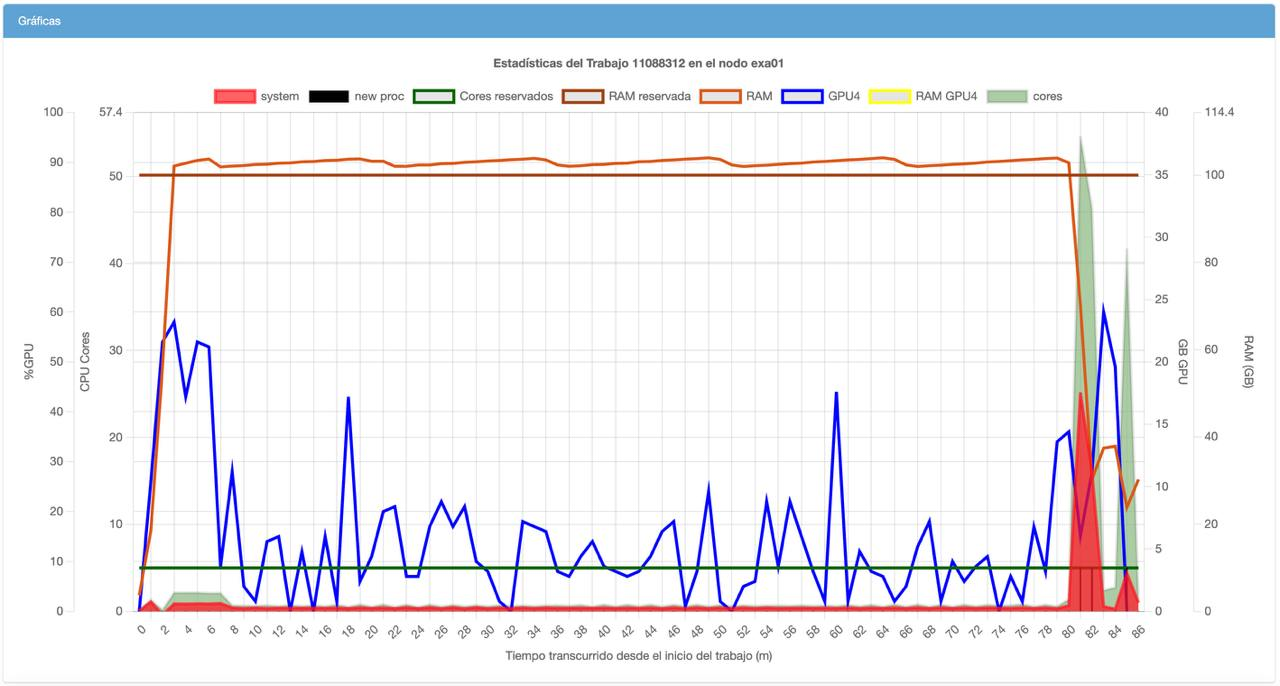
\includegraphics[keepaspectratio]{2d.jpg}}
\caption{Alt text}
\end{figure}

And here is the consumption for \texttt{nnUNet3D}. As we can see, the
resource usage is significantly higher. As we will show later, although
the results are better, the improvement is not substantial enough to
justify this large increase in resource usage.

\begin{figure}
\centering
\pandocbounded{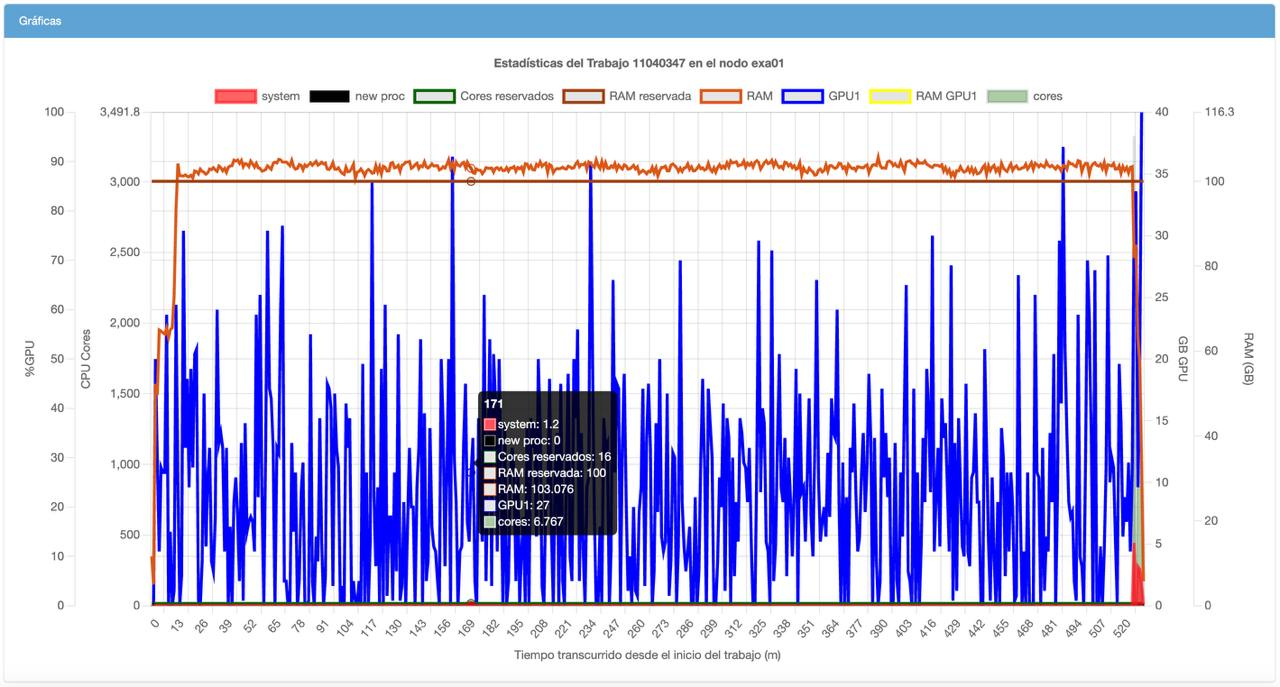
\includegraphics[keepaspectratio]{3d.jpg}}
\caption{Alt text}
\end{figure}

Finally, the training of the YOLO models shows a resource consumption
comparable to \texttt{nnUNet3D}, but as we will see, their performance
is significantly poorer in comparison.

    \subsection{Load the Data}\label{load-the-data}

We have three CSV files containing results: one with only the YOLO model
results, one with the nnUNet results, and one with the combined results.
This separation is necessary because, as we will see later, the results
differ significantly and need to be visualized separately.

    \begin{tcolorbox}[breakable, size=fbox, boxrule=1pt, pad at break*=1mm,colback=cellbackground, colframe=cellborder]
\prompt{In}{incolor}{136}{\boxspacing}
\begin{Verbatim}[commandchars=\\\{\}]
\PY{k+kn}{from}\PY{+w}{ }\PY{n+nn}{SAES}\PY{n+nn}{.}\PY{n+nn}{latex\PYZus{}generation}\PY{n+nn}{.}\PY{n+nn}{stats\PYZus{}table}\PY{+w}{ }\PY{k+kn}{import} \PY{n}{Friedman}\PY{p}{,} \PY{n}{Wilcoxon}\PY{p}{,} \PY{n}{WilcoxonPivot}
\PY{k+kn}{from}\PY{+w}{ }\PY{n+nn}{SAES}\PY{n+nn}{.}\PY{n+nn}{plots}\PY{n+nn}{.}\PY{n+nn}{boxplot}\PY{+w}{ }\PY{k+kn}{import} \PY{n}{Boxplot}
\PY{k+kn}{from}\PY{+w}{ }\PY{n+nn}{SAES}\PY{n+nn}{.}\PY{n+nn}{plots}\PY{n+nn}{.}\PY{n+nn}{CDplot}\PY{+w}{ }\PY{k+kn}{import} \PY{n}{CDplot}
\PY{k+kn}{from}\PY{+w}{ }\PY{n+nn}{SAES}\PY{n+nn}{.}\PY{n+nn}{plots}\PY{n+nn}{.}\PY{n+nn}{violin}\PY{+w}{ }\PY{k+kn}{import} \PY{n}{Violin}
\PY{k+kn}{from}\PY{+w}{ }\PY{n+nn}{SAES}\PY{n+nn}{.}\PY{n+nn}{plots}\PY{n+nn}{.}\PY{n+nn}{HistoPlot}\PY{+w}{ }\PY{k+kn}{import} \PY{n}{HistoPlot}
\PY{k+kn}{from}\PY{+w}{ }\PY{n+nn}{SAES}\PY{n+nn}{.}\PY{n+nn}{plots}\PY{n+nn}{.}\PY{n+nn}{Pplot}\PY{+w}{ }\PY{k+kn}{import} \PY{n}{Pplot}

\PY{k+kn}{import}\PY{+w}{ }\PY{n+nn}{matplotlib}\PY{n+nn}{.}\PY{n+nn}{pyplot}\PY{+w}{ }\PY{k}{as}\PY{+w}{ }\PY{n+nn}{plt}
\PY{k+kn}{from}\PY{+w}{ }\PY{n+nn}{PIL}\PY{+w}{ }\PY{k+kn}{import} \PY{n}{Image}
\PY{k+kn}{import}\PY{+w}{ }\PY{n+nn}{pandas}\PY{+w}{ }\PY{k}{as}\PY{+w}{ }\PY{n+nn}{pd}
\PY{k+kn}{import}\PY{+w}{ }\PY{n+nn}{os}
\end{Verbatim}
\end{tcolorbox}

    \begin{tcolorbox}[breakable, size=fbox, boxrule=1pt, pad at break*=1mm,colback=cellbackground, colframe=cellborder]
\prompt{In}{incolor}{150}{\boxspacing}
\begin{Verbatim}[commandchars=\\\{\}]
\PY{n}{yolo\PYZus{}data} \PY{o}{=} \PY{n}{pd}\PY{o}{.}\PY{n}{read\PYZus{}csv}\PY{p}{(}\PY{l+s+s1}{\PYZsq{}}\PY{l+s+s1}{yolo.csv}\PY{l+s+s1}{\PYZsq{}}\PY{p}{)}
\PY{n}{nnUNet\PYZus{}data} \PY{o}{=} \PY{n}{pd}\PY{o}{.}\PY{n}{read\PYZus{}csv}\PY{p}{(}\PY{l+s+s1}{\PYZsq{}}\PY{l+s+s1}{nnUNet.csv}\PY{l+s+s1}{\PYZsq{}}\PY{p}{)}
\PY{n}{yolo\PYZus{}nnUNet\PYZus{}data} \PY{o}{=} \PY{n}{pd}\PY{o}{.}\PY{n}{read\PYZus{}csv}\PY{p}{(}\PY{l+s+s1}{\PYZsq{}}\PY{l+s+s1}{yolo\PYZus{}nnUNet.csv}\PY{l+s+s1}{\PYZsq{}}\PY{p}{)}

\PY{n}{yolo\PYZus{}nnUNet\PYZus{}data}
\end{Verbatim}
\end{tcolorbox}

            \begin{tcolorbox}[breakable, size=fbox, boxrule=.5pt, pad at break*=1mm, opacityfill=0]
\prompt{Out}{outcolor}{150}{\boxspacing}
\begin{Verbatim}[commandchars=\\\{\}]
     Algorithm Instance MetricName  ExecutionId  MetricValue
0     nnUNet3D    fold1        DSC            1     0.753997
1     nnUNet3D    fold1         FN            1  3086.777778
2     nnUNet3D    fold1        FNR            1     0.237539
3     nnUNet3D    fold1         FP            1  1340.777778
4     nnUNet3D    fold1        FPR            1     0.000186
{\ldots}        {\ldots}      {\ldots}        {\ldots}          {\ldots}          {\ldots}
5095  Yolo2D-s    fold5        DSC           26     0.121399
5096  Yolo2D-s    fold5        DSC           27     0.123975
5097  Yolo2D-s    fold5        DSC           28     0.136433
5098  Yolo2D-s    fold5        DSC           29     0.103208
5099  Yolo2D-s    fold5        DSC           30     0.126677

[5100 rows x 5 columns]
\end{Verbatim}
\end{tcolorbox}
        
    \begin{tcolorbox}[breakable, size=fbox, boxrule=1pt, pad at break*=1mm,colback=cellbackground, colframe=cellborder]
\prompt{In}{incolor}{151}{\boxspacing}
\begin{Verbatim}[commandchars=\\\{\}]
\PY{c+c1}{\PYZsh{} Compared algoritms}
\PY{n}{algorithms} \PY{o}{=} \PY{n}{yolo\PYZus{}nnUNet\PYZus{}data}\PY{o}{.}\PY{n}{Algorithm}
\PY{n+nb}{list}\PY{p}{(}\PY{n}{algorithms}\PY{o}{.}\PY{n}{unique}\PY{p}{(}\PY{p}{)}\PY{p}{)}
\end{Verbatim}
\end{tcolorbox}

            \begin{tcolorbox}[breakable, size=fbox, boxrule=.5pt, pad at break*=1mm, opacityfill=0]
\prompt{Out}{outcolor}{151}{\boxspacing}
\begin{Verbatim}[commandchars=\\\{\}]
['nnUNet3D',
 'nnUNet2D',
 'Yolo3D',
 'Yolo3D-a',
 'Yolo3D-c',
 'Yolo3D-s',
 'Yolo2D',
 'Yolo2D-a',
 'Yolo2D-c',
 'Yolo2D-s']
\end{Verbatim}
\end{tcolorbox}
        
    \begin{tcolorbox}[breakable, size=fbox, boxrule=1pt, pad at break*=1mm,colback=cellbackground, colframe=cellborder]
\prompt{In}{incolor}{ }{\boxspacing}
\begin{Verbatim}[commandchars=\\\{\}]
\PY{c+c1}{\PYZsh{} Load the metrics (quality indicators) data}
\PY{n}{metrics} \PY{o}{=} \PY{n}{pd}\PY{o}{.}\PY{n}{read\PYZus{}csv}\PY{p}{(}\PY{l+s+s1}{\PYZsq{}}\PY{l+s+s1}{metrics.csv}\PY{l+s+s1}{\PYZsq{}}\PY{p}{)}
\PY{n}{metrics}
\end{Verbatim}
\end{tcolorbox}

            \begin{tcolorbox}[breakable, size=fbox, boxrule=.5pt, pad at break*=1mm, opacityfill=0]
\prompt{Out}{outcolor}{ }{\boxspacing}
\begin{Verbatim}[commandchars=\\\{\}]
     MetricName  Maximize
0           DSC      True
1            FN     False
2           FNR     False
3            FP     False
4           FPR     False
5           Iou      True
6           NPV      True
7            TN      True
8            TP      True
9           acc      True
10    precision      True
11       recall      True
12  specificity      True
\end{Verbatim}
\end{tcolorbox}
        
    \subsubsection{Dice Similarity Coefficient
(DSC)}\label{dice-similarity-coefficient-dsc}

The \textbf{Dice Similarity Coefficient (DSC)} is a statistical metric
used to measure the similarity between two sets. In the context of
medical image segmentation, it is commonly used to evaluate the overlap
between the \textbf{predicted segmentation} and the \textbf{ground
truth}.

DSC ranges from 0 to 1: - A DSC of \textbf{1} indicates perfect
agreement (complete overlap). - A DSC of \textbf{0} means no overlap
between the predicted and ground truth regions.

\[
\text{DSC} = \frac{2 \cdot |A \cap B|}{|A| + |B|}
\]

Where: - \(A\) is the set of pixels in the \textbf{ground truth}
segmentation, - \(B\) is the set of pixels in the \textbf{predicted}
segmentation, - \(|A \cap B|\) is the number of overlapping pixels (true
positives), - \(|A|\) and \(|B|\) are the number of pixels in each
respective segmentation mask.

In binary segmentation masks (where 1 = foreground, 0 = background),
this is equivalent to:

\[
\text{DSC} = \frac{2 \cdot TP}{2 \cdot TP + FP + FN}
\]

Where: - \textbf{TP} = True Positives, - \textbf{FP} = False Positives,
- \textbf{FN} = False Negatives.

The Dice coefficient is particularly useful in medical image analysis,
such as MRI segmentation, where class imbalance can be significant and
it is the metric that we will use for our study.

    \begin{tcolorbox}[breakable, size=fbox, boxrule=1pt, pad at break*=1mm,colback=cellbackground, colframe=cellborder]
\prompt{In}{incolor}{140}{\boxspacing}
\begin{Verbatim}[commandchars=\\\{\}]
\PY{n}{metric} \PY{o}{=} \PY{l+s+s2}{\PYZdq{}}\PY{l+s+s2}{DSC}\PY{l+s+s2}{\PYZdq{}}
\end{Verbatim}
\end{tcolorbox}

    \subsection{Boxplot Graph}\label{boxplot-graph}

    A \textbf{boxplot}, also known as a \textbf{box-and-whisker plot}, is a
graphical tool used to summarize and visualize the distribution of a
dataset. It allows you to identify key features such as central
tendency, variability, and the presence of outliers, offering a simple
way to interpret the data.

The \textbf{main body of the boxplot} is the box, which represents the
\textbf{interquartile range (IQR)}, the range between the first quartile
(\textbf{Q1}) and the third quartile (\textbf{Q3}). This area contains
the middle 50\% of the data. Inside the box, a line indicates the
\textbf{median} (second quartile, \textbf{Q2}), the value that divides
the data into two equal halves. The \textbf{whiskers} extend from the
box to the smallest and largest values that are within 1.5 times the IQR
from Q1 or Q3, respectively. Points outside this range are considered
\textbf{outliers} and are often shown as individual points.

The \textbf{interpretation of the boxplot} depends on the context and
the goal of the analysis. If the goal is to \textbf{maximize} a metric
(such as profit or performance), attention should be paid to the higher
values, both within the box and in the upper whiskers or outliers. On
the other hand, if the goal is to \textbf{minimize} (such as errors or
costs), the focus should be on the lower values. Additionally, the
position of the median within the box can indicate the skewness of the
data: if it is closer to Q1 or Q3, the distribution is not symmetrical.

    \begin{tcolorbox}[breakable, size=fbox, boxrule=1pt, pad at break*=1mm,colback=cellbackground, colframe=cellborder]
\prompt{In}{incolor}{ }{\boxspacing}
\begin{Verbatim}[commandchars=\\\{\}]
\PY{n}{boxplot} \PY{o}{=} \PY{n}{Boxplot}\PY{p}{(}\PY{n}{yolo\PYZus{}nnUNet\PYZus{}data}\PY{p}{,} \PY{n}{metrics}\PY{p}{,} \PY{n}{metric}\PY{p}{)}
\PY{n}{boxplot}\PY{o}{.}\PY{n}{show\PYZus{}all\PYZus{}instances}\PY{p}{(}\PY{p}{)}
\end{Verbatim}
\end{tcolorbox}

    \begin{center}
    \adjustimage{max size={0.9\linewidth}{0.9\paperheight}}{SAES_tutorial_files/SAES_tutorial_11_0.png}
    \end{center}
    { \hspace*{\fill} \\}
    
    From this graph, the only clear takeaway is that the nnUNet models
significantly outperform the YOLO models. Therefore, we will analyze
them separately.

\subsubsection{Boxplot YOLO}\label{boxplot-yolo}

    \begin{tcolorbox}[breakable, size=fbox, boxrule=1pt, pad at break*=1mm,colback=cellbackground, colframe=cellborder]
\prompt{In}{incolor}{ }{\boxspacing}
\begin{Verbatim}[commandchars=\\\{\}]
\PY{n}{boxplot} \PY{o}{=} \PY{n}{Boxplot}\PY{p}{(}\PY{n}{yolo\PYZus{}data}\PY{p}{,} \PY{n}{metrics}\PY{p}{,} \PY{n}{metric}\PY{p}{)}
\PY{n}{boxplot}\PY{o}{.}\PY{n}{show\PYZus{}all\PYZus{}instances}\PY{p}{(}\PY{p}{)}
\end{Verbatim}
\end{tcolorbox}

    \begin{center}
    \adjustimage{max size={0.9\linewidth}{0.9\paperheight}}{SAES_tutorial_files/SAES_tutorial_13_0.png}
    \end{center}
    { \hspace*{\fill} \\}
    
    This boxplot clearly shows a consistent winner across every fold of
validation: Yolo2D, which uses a consensus approach over three models,
each trained on a single anatomical plane. The conclusion we can draw is
that, due to the inherently 2D nature of the YOLO architecture, its
performance significantly improves when it is trained on images from
only one plane at a time. Once a consensus is formed among the three
specialized models, the overall performance becomes even better.

This interpretation is further supported by the fact that all the 2D
models outperform any of the 3D models, according to the graph. This
suggests that when using a 2D-based model architecture, attempting to
learn from 3D information directly is suboptimal. Instead, the learning
process should be divided across multiple models, each focusing on a
specific 2D slice or view of the data.

\subsubsection{Boxplot nnUNet}\label{boxplot-nnunet}

    \begin{tcolorbox}[breakable, size=fbox, boxrule=1pt, pad at break*=1mm,colback=cellbackground, colframe=cellborder]
\prompt{In}{incolor}{154}{\boxspacing}
\begin{Verbatim}[commandchars=\\\{\}]
\PY{n}{boxplot} \PY{o}{=} \PY{n}{Boxplot}\PY{p}{(}\PY{n}{nnUNet\PYZus{}data}\PY{p}{,} \PY{n}{metrics}\PY{p}{,} \PY{n}{metric}\PY{p}{)}
\PY{n}{boxplot}\PY{o}{.}\PY{n}{show\PYZus{}all\PYZus{}instances}\PY{p}{(}\PY{p}{)}
\end{Verbatim}
\end{tcolorbox}

    \begin{center}
    \adjustimage{max size={0.9\linewidth}{0.9\paperheight}}{SAES_tutorial_files/SAES_tutorial_15_0.png}
    \end{center}
    { \hspace*{\fill} \\}
    
    The results of the nnUNet models are easier to interpret. The 3D version
achieves a Dice Similarity Coefficient (DSC) of around 0.76, while the
2D version scores around 0.72. This 0.06 difference can be considered
significant, depending on how strict we want to be. However, if we are
willing to sacrifice a bit of precision, the 2D version is a very
attractive option, as its training process is approximately 10 times
cheaper.

    \subsection{Violin Plot}\label{violin-plot}

A \textbf{violin plot} is another graphical tool used to visualize the
distribution of a dataset, combining aspects of both a \textbf{boxplot}
and a \textbf{density plot}. It is particularly useful for understanding
the distribution of data, especially when comparing multiple groups or
datasets.

The \textbf{main feature of a violin plot} is its \textbf{shape}, which
is formed by a \textbf{kernel density estimation (KDE)} that shows the
probability distribution of the data. The plot looks like a violin
because it is symmetric on both sides of a central axis, with the width
at different values indicating the density of data points at that value.

Here are the key components of a violin plot:

\begin{enumerate}
\def\labelenumi{\arabic{enumi}.}
\item
  \textbf{Central axis}: Like a boxplot, a violin plot has a central
  axis where the data is plotted. This axis typically represents the
  variable of interest.
\item
  \textbf{Density curve (the ``violin'' shape)}: The main part of the
  violin plot is the \textbf{density curve}, which shows how the data is
  distributed along the axis. Wider sections of the curve indicate
  higher density (more data points), while narrower sections indicate
  lower density (fewer data points). The shape helps to visualize the
  distribution more clearly than a boxplot alone, especially when there
  are multiple peaks (modes) in the data.
\item
  \textbf{Boxplot within the violin}: A \textbf{boxplot} is often
  included inside the violin plot, showing the \textbf{median},
  \textbf{first quartile (Q1)}, and \textbf{third quartile (Q3)}. The
  whiskers of the boxplot often extend to the smallest and largest
  values within 1.5 times the IQR, and any data points outside this
  range are considered outliers.
\item
  \textbf{Individual data points (optional)}: Some violin plots also
  show individual data points as dots or other markers, providing an
  additional layer of detail.
\end{enumerate}

\subsubsection{\texorpdfstring{\textbf{Interpretation of a Violin
Plot}:}{Interpretation of a Violin Plot:}}\label{interpretation-of-a-violin-plot}

\begin{itemize}
\tightlist
\item
  \textbf{Shape}: The overall shape of the violin gives insights into
  the distribution of the data. A symmetrical violin suggests a roughly
  normal distribution, while asymmetrical shapes can indicate skewness.
\item
  \textbf{Peaks}: The presence of multiple peaks in the violin indicates
  that the data may have multiple modes, or subgroups, within it.
\item
  \textbf{Width}: The width of the violin at various values provides a
  clear indication of the data's \textbf{density}---wider areas mean
  higher data concentration, and narrower areas mean less concentration.
\item
  \textbf{Boxplot features}: The boxplot part of the violin allows you
  to see the \textbf{median}, \textbf{quartiles}, and \textbf{outliers},
  giving a summary of the spread and central tendency of the data.
\end{itemize}

Violin plots are particularly useful when comparing multiple
distributions side-by-side, as they provide both a summary and a
detailed visualization of the data's distribution.

    \begin{tcolorbox}[breakable, size=fbox, boxrule=1pt, pad at break*=1mm,colback=cellbackground, colframe=cellborder]
\prompt{In}{incolor}{156}{\boxspacing}
\begin{Verbatim}[commandchars=\\\{\}]
\PY{n}{violin} \PY{o}{=} \PY{n}{Violin}\PY{p}{(}\PY{n}{yolo\PYZus{}nnUNet\PYZus{}data}\PY{p}{,} \PY{n}{metrics}\PY{p}{,} \PY{l+s+s2}{\PYZdq{}}\PY{l+s+s2}{DSC}\PY{l+s+s2}{\PYZdq{}}\PY{p}{)}
\PY{n}{violin}\PY{o}{.}\PY{n}{show\PYZus{}all\PYZus{}instances}\PY{p}{(}\PY{p}{)}
\end{Verbatim}
\end{tcolorbox}

    \begin{center}
    \adjustimage{max size={0.9\linewidth}{0.9\paperheight}}{SAES_tutorial_files/SAES_tutorial_18_0.png}
    \end{center}
    { \hspace*{\fill} \\}
    
    \subsubsection{Violin Plot Yolo}\label{violin-plot-yolo}

    \begin{tcolorbox}[breakable, size=fbox, boxrule=1pt, pad at break*=1mm,colback=cellbackground, colframe=cellborder]
\prompt{In}{incolor}{157}{\boxspacing}
\begin{Verbatim}[commandchars=\\\{\}]
\PY{n}{violin} \PY{o}{=} \PY{n}{Violin}\PY{p}{(}\PY{n}{yolo\PYZus{}data}\PY{p}{,} \PY{n}{metrics}\PY{p}{,} \PY{l+s+s2}{\PYZdq{}}\PY{l+s+s2}{DSC}\PY{l+s+s2}{\PYZdq{}}\PY{p}{)}
\PY{n}{violin}\PY{o}{.}\PY{n}{show\PYZus{}all\PYZus{}instances}\PY{p}{(}\PY{p}{)}
\end{Verbatim}
\end{tcolorbox}

    \begin{center}
    \adjustimage{max size={0.9\linewidth}{0.9\paperheight}}{SAES_tutorial_files/SAES_tutorial_20_0.png}
    \end{center}
    { \hspace*{\fill} \\}
    
    \subsubsection{Violin Plot nnUNet}\label{violin-plot-nnunet}

    \begin{tcolorbox}[breakable, size=fbox, boxrule=1pt, pad at break*=1mm,colback=cellbackground, colframe=cellborder]
\prompt{In}{incolor}{158}{\boxspacing}
\begin{Verbatim}[commandchars=\\\{\}]
\PY{n}{violin} \PY{o}{=} \PY{n}{Violin}\PY{p}{(}\PY{n}{nnUNet\PYZus{}data}\PY{p}{,} \PY{n}{metrics}\PY{p}{,} \PY{l+s+s2}{\PYZdq{}}\PY{l+s+s2}{DSC}\PY{l+s+s2}{\PYZdq{}}\PY{p}{)}
\PY{n}{violin}\PY{o}{.}\PY{n}{show\PYZus{}all\PYZus{}instances}\PY{p}{(}\PY{p}{)}
\end{Verbatim}
\end{tcolorbox}

    \begin{center}
    \adjustimage{max size={0.9\linewidth}{0.9\paperheight}}{SAES_tutorial_files/SAES_tutorial_22_0.png}
    \end{center}
    { \hspace*{\fill} \\}
    
    \subsection{HistPlot}\label{histplot}

A \textbf{histogram} (or \textbf{histoplot}) is another graphical
representation used to summarize the distribution of a dataset, but it
differs from a boxplot in how it organizes and displays the data.

In a \textbf{histogram}, the data is divided into \textbf{bins} or
\textbf{intervals}, and the frequency of data points within each
interval is represented by the height of a bar. The \textbf{x-axis}
represents the values or ranges of the dataset (the bins), while the
\textbf{y-axis} represents the frequency or count of data points within
each bin. This type of plot is particularly useful for understanding the
\textbf{shape} of the data distribution, including whether the data is
\textbf{skewed}, \textbf{normal}, or exhibits any other patterns.

\subsubsection{Key Features of a
Histogram:}\label{key-features-of-a-histogram}

\begin{enumerate}
\def\labelenumi{\arabic{enumi}.}
\item
  \textbf{Bins}: The data is grouped into bins, and the number of bins
  can affect the appearance of the histogram. Too few bins may
  oversimplify the distribution, while too many bins may make the plot
  noisy and harder to interpret. The size of the bins often depends on
  the range of the data and the level of detail desired.
\item
  \textbf{Frequency}: The height of each bar corresponds to the number
  of data points within that bin. A taller bar indicates a higher
  frequency of data in that range.
\item
  \textbf{Shape of Distribution}: The histogram visually reveals the
  overall shape of the distribution. For example, a bell-shaped
  histogram suggests that the data is normally distributed, while a
  skewed histogram indicates that the data is not symmetrically
  distributed.
\item
  \textbf{Outliers}: Unlike the boxplot, histograms don't explicitly
  highlight outliers, but you can identify outliers as bins with
  significantly lower frequencies compared to neighboring bins. If a bin
  is far from the main body of the distribution, it might suggest the
  presence of unusual data points.
\end{enumerate}

\subsubsection{Interpretation:}\label{interpretation}

\begin{itemize}
\item
  \textbf{Skewness}: If the histogram's tail is stretched out on the
  right, it suggests \textbf{right skewness} (or positive skew),
  indicating that the data has more values on the lower end but some
  very high values. Conversely, if the tail is stretched out on the
  left, it suggests \textbf{left skewness} (or negative skew).
\item
  \textbf{Peaks}: A histogram with one peak is \textbf{unimodal}, while
  one with multiple peaks could be \textbf{multimodal}, suggesting that
  the dataset may consist of more than one underlying distribution.
\item
  \textbf{Central Tendency}: You can visually identify the central
  tendency (such as the mean or median) by looking at where the majority
  of the data is concentrated. In symmetric distributions, the mean and
  median are close to each other.
\item
  \textbf{Spread}: The width of the histogram gives an idea of the
  spread of the data. A wider histogram indicates more variability,
  while a narrower one suggests that the data points are more tightly
  grouped around the central tendency.
\end{itemize}

    \begin{tcolorbox}[breakable, size=fbox, boxrule=1pt, pad at break*=1mm,colback=cellbackground, colframe=cellborder]
\prompt{In}{incolor}{159}{\boxspacing}
\begin{Verbatim}[commandchars=\\\{\}]
\PY{n}{histoplot} \PY{o}{=} \PY{n}{HistoPlot}\PY{p}{(}\PY{n}{yolo\PYZus{}nnUNet\PYZus{}data}\PY{p}{,} \PY{n}{metrics}\PY{p}{,} \PY{l+s+s2}{\PYZdq{}}\PY{l+s+s2}{DSC}\PY{l+s+s2}{\PYZdq{}}\PY{p}{)}
\PY{n}{histoplot}\PY{o}{.}\PY{n}{show\PYZus{}all\PYZus{}instances}\PY{p}{(}\PY{p}{)}
\end{Verbatim}
\end{tcolorbox}

    \begin{center}
    \adjustimage{max size={0.9\linewidth}{0.9\paperheight}}{SAES_tutorial_files/SAES_tutorial_24_0.png}
    \end{center}
    { \hspace*{\fill} \\}
    
    \subsubsection{HistPlot Yolo}\label{histplot-yolo}

    \begin{tcolorbox}[breakable, size=fbox, boxrule=1pt, pad at break*=1mm,colback=cellbackground, colframe=cellborder]
\prompt{In}{incolor}{160}{\boxspacing}
\begin{Verbatim}[commandchars=\\\{\}]
\PY{n}{histoplot} \PY{o}{=} \PY{n}{HistoPlot}\PY{p}{(}\PY{n}{yolo\PYZus{}data}\PY{p}{,} \PY{n}{metrics}\PY{p}{,} \PY{l+s+s2}{\PYZdq{}}\PY{l+s+s2}{DSC}\PY{l+s+s2}{\PYZdq{}}\PY{p}{)}
\PY{n}{histoplot}\PY{o}{.}\PY{n}{show\PYZus{}all\PYZus{}instances}\PY{p}{(}\PY{p}{)}
\end{Verbatim}
\end{tcolorbox}

    \begin{center}
    \adjustimage{max size={0.9\linewidth}{0.9\paperheight}}{SAES_tutorial_files/SAES_tutorial_26_0.png}
    \end{center}
    { \hspace*{\fill} \\}
    
    \subsubsection{HistPlot nnUNet}\label{histplot-nnunet}

    \begin{tcolorbox}[breakable, size=fbox, boxrule=1pt, pad at break*=1mm,colback=cellbackground, colframe=cellborder]
\prompt{In}{incolor}{161}{\boxspacing}
\begin{Verbatim}[commandchars=\\\{\}]
\PY{n}{histoplot} \PY{o}{=} \PY{n}{HistoPlot}\PY{p}{(}\PY{n}{nnUNet\PYZus{}data}\PY{p}{,} \PY{n}{metrics}\PY{p}{,} \PY{l+s+s2}{\PYZdq{}}\PY{l+s+s2}{DSC}\PY{l+s+s2}{\PYZdq{}}\PY{p}{)}
\PY{n}{histoplot}\PY{o}{.}\PY{n}{show\PYZus{}all\PYZus{}instances}\PY{p}{(}\PY{p}{)}
\end{Verbatim}
\end{tcolorbox}

    \begin{center}
    \adjustimage{max size={0.9\linewidth}{0.9\paperheight}}{SAES_tutorial_files/SAES_tutorial_28_0.png}
    \end{center}
    { \hspace*{\fill} \\}
    
    \subsection{Critical Distance Graph}\label{critical-distance-graph}

    A critical distance (CD) graph is used to compare the performance of
multiple algorithms statistically. It is typically generated using the
Nemenyi test, which is a post-hoc test applied after a Friedman test has
shown significant differences between algorithms.

In this graph: - Each algorithm is assigned a rank based on its
performance on a metric (e.g., accuracy, hypervolume, etc.) across
multiple datasets or experiments. - The average rank of each algorithm
is plotted on a horizontal axis. - A critical distance (CD) value is
calculated, representing the threshold for statistically significant
differences between algorithm ranks. - Algorithms connected by
horizontal lines are statistically indistinguishable within the critical
distance, meaning their performance differences are not significant at
the chosen confidence level.

    \begin{tcolorbox}[breakable, size=fbox, boxrule=1pt, pad at break*=1mm,colback=cellbackground, colframe=cellborder]
\prompt{In}{incolor}{162}{\boxspacing}
\begin{Verbatim}[commandchars=\\\{\}]
\PY{n}{cdplot} \PY{o}{=} \PY{n}{CDplot}\PY{p}{(}\PY{n}{yolo\PYZus{}nnUNet\PYZus{}data}\PY{p}{,} \PY{n}{metrics}\PY{p}{,} \PY{l+s+s1}{\PYZsq{}}\PY{l+s+s1}{DSC}\PY{l+s+s1}{\PYZsq{}}\PY{p}{)}
\PY{n}{cdplot}\PY{o}{.}\PY{n}{show}\PY{p}{(}\PY{p}{)}
\end{Verbatim}
\end{tcolorbox}

    \begin{center}
    \adjustimage{max size={0.9\linewidth}{0.9\paperheight}}{SAES_tutorial_files/SAES_tutorial_31_0.png}
    \end{center}
    { \hspace*{\fill} \\}
    
    \subsubsection{Critical Distance Graph
Results}\label{critical-distance-graph-results}

As expected, the Critical Distance Graph displays, in order, which were
the \textbf{best-performing models}:

\begin{enumerate}
\def\labelenumi{\arabic{enumi}.}
\tightlist
\item
  �� \textbf{nnUNet3D}
\item
  �� \textbf{nnUNet2D}
\item
  \textbf{Yolo2D}
\item
  \emph{Yolo2D-s}
\item
  \emph{Yolo2D-c}
\item
  \emph{Yolo2D-a}
\item
  \emph{Yolo3D-a}
\item
  \emph{Yolo3D-c}
\item
  \emph{Yolo3D-s}
\item
  \textbf{Yolo3D}
\end{enumerate}

\begin{quote}
✅ This ranking confirms expected performance trends across the tested
architectures.
\end{quote}

    \subsection{LaTeX report Generation}\label{latex-report-generation}

    Lastly, we offer a variety of LaTeX reports tailored for different
purposes, including scientific articles and presentations (take into
account that only the .tex source code is provided and you will need an
external tool like overleaf to render the LaTeX code into pdf format).
Below are the four types of LaTeX reports you can generate, along with a
brief explanation of each:

\subsubsection{Median Table with Friedman Test}
\begin{itemize}
  \tightlist
  \item
    \textbf{Description}: Extends the median table by incorporating the
    Friedman test results.\\
  \item
    \textbf{Purpose}: Highlights significant differences among multiple
    groups or algorithms, assuming a non-parametric distribution.\\
  \item
    \textbf{Use Case}: Ideal for analyzing and reporting results where
    ranking of methods or treatments is necessary.
  \end{itemize}
\begin{table}[H]
        \caption{DSC.  Median and Interquartile Range Friedman base Table (+ implies that the difference between the algorithms for the instance in the select row is significant)
}
        \vspace{1mm}
        \centering
        \begin{scriptsize}
        \begin{tabular}{l|c|c|c|c|c|c|c|c|c|c|c}
        \hline
        & nnUNet3D & nnUNet2D & Yolo3D & Yolo3D-a & Yolo3D-c & Yolo3D-s & Yolo2D & Yolo2D-a & Yolo2D-c & Yolo2D-s & FT \\ \hline
fold1 & \cellcolor{gray95}$\SI{7.57e-01}{}_{ \SI{8.00e-03}{} }$ & \cellcolor{gray25}$\SI{7.14e-01}{}_{ \SI{1.03e-02}{} }$ & $\SI{8.99e-02}{}_{ \SI{8.32e-03}{} }$ & $\SI{9.36e-02}{}_{ \SI{6.00e-03}{} }$ & $\SI{8.90e-02}{}_{ \SI{2.03e-03}{} }$ & $\SI{8.98e-02}{}_{ \SI{1.87e-03}{} }$ & $\SI{1.32e-01}{}_{ \SI{9.79e-03}{} }$ & $\SI{1.20e-01}{}_{ \SI{1.02e-02}{} }$ & $\SI{1.20e-01}{}_{ \SI{2.25e-03}{} }$ & $\SI{1.22e-01}{}_{ \SI{7.66e-03}{} }$ & + \\ 
fold2 & \cellcolor{gray95}$\SI{6.77e-01}{}_{ \SI{1.96e-02}{} }$ & \cellcolor{gray25}$\SI{5.94e-01}{}_{ \SI{1.60e-02}{} }$ & $\SI{8.69e-02}{}_{ \SI{1.03e-02}{} }$ & $\SI{1.18e-01}{}_{ \SI{8.94e-03}{} }$ & $\SI{1.09e-01}{}_{ \SI{1.28e-02}{} }$ & $\SI{1.09e-01}{}_{ \SI{1.81e-03}{} }$ & $\SI{1.46e-01}{}_{ \SI{4.88e-03}{} }$ & $\SI{1.13e-01}{}_{ \SI{8.82e-04}{} }$ & $\SI{1.13e-01}{}_{ \SI{1.07e-03}{} }$ & $\SI{1.24e-01}{}_{ \SI{5.70e-04}{} }$ & + \\ 
fold3 & \cellcolor{gray95}$\SI{7.03e-01}{}_{ \SI{6.58e-03}{} }$ & \cellcolor{gray25}$\SI{6.78e-01}{}_{ \SI{1.08e-02}{} }$ & $\SI{1.39e-01}{}_{ \SI{2.68e-03}{} }$ & $\SI{1.29e-01}{}_{ \SI{1.07e-02}{} }$ & $\SI{1.38e-01}{}_{ \SI{8.34e-03}{} }$ & $\SI{1.51e-01}{}_{ \SI{2.52e-03}{} }$ & $\SI{1.69e-01}{}_{ \SI{2.00e-03}{} }$ & $\SI{1.47e-01}{}_{ \SI{7.99e-03}{} }$ & $\SI{1.58e-01}{}_{ \SI{8.80e-03}{} }$ & $\SI{1.60e-01}{}_{ \SI{9.26e-03}{} }$ & + \\ 
fold4 & \cellcolor{gray95}$\SI{7.75e-01}{}_{ \SI{6.24e-03}{} }$ & \cellcolor{gray25}$\SI{7.39e-01}{}_{ \SI{6.19e-03}{} }$ & $\SI{3.47e-02}{}_{ \SI{2.81e-03}{} }$ & $\SI{4.14e-02}{}_{ \SI{6.73e-04}{} }$ & $\SI{3.67e-02}{}_{ \SI{2.35e-03}{} }$ & $\SI{3.67e-02}{}_{ \SI{4.16e-03}{} }$ & $\SI{6.22e-02}{}_{ \SI{2.49e-03}{} }$ & $\SI{4.41e-02}{}_{ \SI{3.03e-03}{} }$ & $\SI{4.37e-02}{}_{ \SI{3.43e-03}{} }$ & $\SI{4.62e-02}{}_{ \SI{3.39e-03}{} }$ & + \\ 
fold5 & \cellcolor{gray95}$\SI{7.65e-01}{}_{ \SI{6.24e-03}{} }$ & \cellcolor{gray25}$\SI{7.31e-01}{}_{ \SI{6.65e-03}{} }$ & $\SI{6.02e-02}{}_{ \SI{6.44e-03}{} }$ & $\SI{7.06e-02}{}_{ \SI{8.53e-03}{} }$ & $\SI{7.53e-02}{}_{ \SI{3.54e-03}{} }$ & $\SI{6.74e-02}{}_{ \SI{2.66e-03}{} }$ & $\SI{1.31e-01}{}_{ \SI{2.02e-03}{} }$ & $\SI{1.02e-01}{}_{ \SI{6.22e-03}{} }$ & $\SI{1.04e-01}{}_{ \SI{8.58e-04}{} }$ & $\SI{1.21e-01}{}_{ \SI{1.21e-02}{} }$ & + \\ 

        \end{tabular}
        \end{scriptsize}
        \end{table}
\subsubsection{Median Table with Wilcoxon Pairwise Test (Pivot-Based)}
\begin{itemize}
  \tightlist
  \item
    \textbf{Description}: Combines the median table with the results of
    Wilcoxon signed-rank pairwise tests using a pivot-based approach.\\
  \item
    \textbf{Purpose}: Provides insights into pairwise comparisons of the
    experimental groups relative to a designated pivot group.\\
  \item
    \textbf{Use Case}: Valuable for scenarios requiring focused
    comparisons against a baseline or reference algorithm.
  \end{itemize}
\begin{table}[H]
        \caption{DSC.  Median and Interquartile Range Wilcoxon Pivot Table (- implies that the pivot algorithm (last column) is statistically worse, = indicates that the differences are not significant.)
}
        \vspace{1mm}
        \centering
        \begin{scriptsize}
        \begin{tabular}{l|c|c|c|c|c|c|c|c|c|c}
        \hline
        & nnUNet3D & nnUNet2D & Yolo3D & Yolo3D-a & Yolo3D-c & Yolo3D-s & Yolo2D & Yolo2D-a & Yolo2D-c & Yolo2D-s \\ \hline
fold1 & \cellcolor{gray95}$\SI{7.57e-01}{}_{ \SI{8.00e-03}{} } -$ & \cellcolor{gray25}$\SI{7.14e-01}{}_{ \SI{1.03e-02}{} } -$ & $\SI{8.99e-02}{}_{ \SI{8.32e-03}{} } +$ & $\SI{9.36e-02}{}_{ \SI{6.00e-03}{} } +$ & $\SI{8.90e-02}{}_{ \SI{2.03e-03}{} } +$ & $\SI{8.98e-02}{}_{ \SI{1.87e-03}{} } +$ & $\SI{1.32e-01}{}_{ \SI{9.79e-03}{} } -$ & $\SI{1.20e-01}{}_{ \SI{1.02e-02}{} } =$ & $\SI{1.20e-01}{}_{ \SI{2.25e-03}{} } =$ & $\SI{1.22e-01}{}_{ \SI{7.66e-03}{} } $ \\ 
fold2 & \cellcolor{gray95}$\SI{6.77e-01}{}_{ \SI{1.96e-02}{} } -$ & \cellcolor{gray25}$\SI{5.94e-01}{}_{ \SI{1.60e-02}{} } -$ & $\SI{8.69e-02}{}_{ \SI{1.03e-02}{} } +$ & $\SI{1.18e-01}{}_{ \SI{8.94e-03}{} } +$ & $\SI{1.09e-01}{}_{ \SI{1.28e-02}{} } +$ & $\SI{1.09e-01}{}_{ \SI{1.81e-03}{} } +$ & $\SI{1.46e-01}{}_{ \SI{4.88e-03}{} } -$ & $\SI{1.13e-01}{}_{ \SI{8.82e-04}{} } +$ & $\SI{1.13e-01}{}_{ \SI{1.07e-03}{} } +$ & $\SI{1.24e-01}{}_{ \SI{5.70e-04}{} } $ \\ 
fold3 & \cellcolor{gray95}$\SI{7.03e-01}{}_{ \SI{6.58e-03}{} } -$ & \cellcolor{gray25}$\SI{6.78e-01}{}_{ \SI{1.08e-02}{} } -$ & $\SI{1.39e-01}{}_{ \SI{2.68e-03}{} } +$ & $\SI{1.29e-01}{}_{ \SI{1.07e-02}{} } +$ & $\SI{1.38e-01}{}_{ \SI{8.34e-03}{} } +$ & $\SI{1.51e-01}{}_{ \SI{2.52e-03}{} } +$ & $\SI{1.69e-01}{}_{ \SI{2.00e-03}{} } -$ & $\SI{1.47e-01}{}_{ \SI{7.99e-03}{} } +$ & $\SI{1.58e-01}{}_{ \SI{8.80e-03}{} } =$ & $\SI{1.60e-01}{}_{ \SI{9.26e-03}{} } $ \\ 
fold4 & \cellcolor{gray95}$\SI{7.75e-01}{}_{ \SI{6.24e-03}{} } -$ & \cellcolor{gray25}$\SI{7.39e-01}{}_{ \SI{6.19e-03}{} } -$ & $\SI{3.47e-02}{}_{ \SI{2.81e-03}{} } +$ & $\SI{4.14e-02}{}_{ \SI{6.73e-04}{} } +$ & $\SI{3.67e-02}{}_{ \SI{2.35e-03}{} } +$ & $\SI{3.67e-02}{}_{ \SI{4.16e-03}{} } +$ & $\SI{6.22e-02}{}_{ \SI{2.49e-03}{} } -$ & $\SI{4.41e-02}{}_{ \SI{3.03e-03}{} } +$ & $\SI{4.37e-02}{}_{ \SI{3.43e-03}{} } +$ & $\SI{4.62e-02}{}_{ \SI{3.39e-03}{} } $ \\ 
fold5 & \cellcolor{gray95}$\SI{7.65e-01}{}_{ \SI{6.24e-03}{} } -$ & \cellcolor{gray25}$\SI{7.31e-01}{}_{ \SI{6.65e-03}{} } -$ & $\SI{6.02e-02}{}_{ \SI{6.44e-03}{} } +$ & $\SI{7.06e-02}{}_{ \SI{8.53e-03}{} } +$ & $\SI{7.53e-02}{}_{ \SI{3.54e-03}{} } +$ & $\SI{6.74e-02}{}_{ \SI{2.66e-03}{} } +$ & $\SI{1.31e-01}{}_{ \SI{2.02e-03}{} } -$ & $\SI{1.02e-01}{}_{ \SI{6.22e-03}{} } +$ & $\SI{1.04e-01}{}_{ \SI{8.58e-04}{} } +$ & $\SI{1.21e-01}{}_{ \SI{1.21e-02}{} } $ \\ 
\hline + / - / = & \textbf0 / \textbf5 / \textbf0 & \textbf0 / \textbf5 / \textbf0 & \textbf5 / \textbf0 / \textbf0 & \textbf5 / \textbf0 / \textbf0 & \textbf5 / \textbf0 / \textbf0 & \textbf5 / \textbf0 / \textbf0 & \textbf0 / \textbf5 / \textbf0 & \textbf4 / \textbf0 / \textbf1 & \textbf3 / \textbf0 / \textbf2
        \end{tabular}
        \end{scriptsize}
        \end{table}
\subsubsection{Pairwise Wilcoxon Test Table (1-to-1 Comparison)}

\begin{itemize}
  \tightlist
  \item
    \textbf{Description}: Presents pairwise Wilcoxon signed-rank test
    results for direct 1-to-1 comparisons between groups.\\
  \item
    \textbf{Purpose}: Offers detailed insights into individual pair
    comparisons without the need for a pivot.\\
  \item
    \textbf{Use Case}: Suitable for comprehensive pairwise statistical
    analysis in experimental studies.
  \end{itemize}
\begin{table}[H]
        \caption{DSC.  Wilcoxon Test 1vs1 Table. Each symbol in the cells represents a problem. Symbol - indicates that the row algorithm performs worse with statistical confidence;  symbol = implies that the differences are not significant. Instances (in order) : ['fold1' 'fold2' 'fold3' 'fold4' 'fold5']
}
        \vspace{1mm}
        \centering
        \begin{scriptsize}
        \begin{tabular}{l|c|c|c|c|c|c|c|c|c}
        \hline
        & nnUNet2D & Yolo3D & Yolo3D-a & Yolo3D-c & Yolo3D-s & Yolo2D & Yolo2D-a & Yolo2D-c & Yolo2D-s \\ \hline
nnUNet3D & \texttt{+++++} & \texttt{+++++} & \texttt{+++++} & \texttt{+++++} & \texttt{+++++} & \texttt{+++++} & \texttt{+++++} & \texttt{+++++} & \texttt{+++++} \\
nnUNet2D &  & \texttt{+++++} & \texttt{+++++} & \texttt{+++++} & \texttt{+++++} & \texttt{+++++} & \texttt{+++++} & \texttt{+++++} & \texttt{+++++} \\
Yolo3D & \texttt{} &  & \texttt{--+--} & \texttt{=-=--} & \texttt{=--=-} & \texttt{-----} & \texttt{-----} & \texttt{-----} & \texttt{-----} \\
Yolo3D-a & \texttt{} & \texttt{} &  & \texttt{++-+-} & \texttt{++-++} & \texttt{-----} & \texttt{-+---} & \texttt{-+---} & \texttt{-----} \\
Yolo3D-c & \texttt{} & \texttt{} & \texttt{} &  & \texttt{-=-=+} & \texttt{-----} & \texttt{-=---} & \texttt{-=---} & \texttt{-----} \\
Yolo3D-s & \texttt{} & \texttt{} & \texttt{} & \texttt{} &  & \texttt{-----} & \texttt{--+--} & \texttt{-----} & \texttt{-----} \\
Yolo2D & \texttt{} & \texttt{} & \texttt{} & \texttt{} & \texttt{} &  & \texttt{+++++} & \texttt{+++++} & \texttt{+++++} \\
Yolo2D-a & \texttt{} & \texttt{} & \texttt{} & \texttt{} & \texttt{} & \texttt{} &  & \texttt{=--=-} & \texttt{=----} \\
Yolo2D-c & \texttt{} & \texttt{} & \texttt{} & \texttt{} & \texttt{} & \texttt{} & \texttt{} &  & \texttt{=-=--} \\

        \end{tabular}
        \end{scriptsize}
        \end{table}
    \subsection{Bayesian Posterior Plot}\label{bayesian-posterior-plot}

The graph is a \textbf{ternary plot}, which is used to visualize
probabilistic comparisons among three categories. In the context of
Bayesian statistical tests, ternary plots are often employed to compare
the relative performance of two competing algorithms while also
accounting for the possibility of no significant difference.

Each point in the ternary plot represents a comparison outcome from a
statistical test, where:

\begin{itemize}
\tightlist
\item
  One axis represents the probability that \textbf{Algorithm A is
  better}.
\item
  Another axis represents the probability that \textbf{Algorithm B is
  better}.
\item
  The third axis represents the probability that \textbf{there is no
  meaningful difference} between the two.
\end{itemize}

The color intensity in the graph typically represents the density of
points, indicating how often different probability distributions occur.

\subsubsection{Bayesian Sign Test}\label{bayesian-sign-test}

\begin{itemize}
\tightlist
\item
  The Bayesian Sign Test is a \textbf{simpler} statistical method that
  assesses the probability that one algorithm is better than another
  based on direct pairwise comparisons.
\item
  It only considers \textbf{the direction of differences} (i.e., which
  algorithm performs better), ignoring the magnitude of the differences.
\item
  It assumes that the comparisons are independent and does not account
  for the distribution of the differences.
\end{itemize}

    \begin{tcolorbox}[breakable, size=fbox, boxrule=1pt, pad at break*=1mm,colback=cellbackground, colframe=cellborder]
\prompt{In}{incolor}{163}{\boxspacing}
\begin{Verbatim}[commandchars=\\\{\}]
\PY{n}{metric} \PY{o}{=} \PY{l+s+s2}{\PYZdq{}}\PY{l+s+s2}{DSC}\PY{l+s+s2}{\PYZdq{}}
\PY{n}{pivot} \PY{o}{=} \PY{l+s+s2}{\PYZdq{}}\PY{l+s+s2}{Yolo2D}\PY{l+s+s2}{\PYZdq{}}
\PY{n}{sign} \PY{o}{=} \PY{n}{Pplot}\PY{p}{(}\PY{n}{yolo\PYZus{}data}\PY{p}{,} \PY{n}{metrics}\PY{p}{,} \PY{n}{metric}\PY{p}{,} \PY{n}{bayesian\PYZus{}test}\PY{o}{=}\PY{l+s+s2}{\PYZdq{}}\PY{l+s+s2}{sign}\PY{l+s+s2}{\PYZdq{}}\PY{p}{)}
\PY{n}{rank} \PY{o}{=} \PY{n}{Pplot}\PY{p}{(}\PY{n}{yolo\PYZus{}data}\PY{p}{,} \PY{n}{metrics}\PY{p}{,} \PY{n}{metric}\PY{p}{,} \PY{n}{bayesian\PYZus{}test}\PY{o}{=}\PY{l+s+s2}{\PYZdq{}}\PY{l+s+s2}{rank}\PY{l+s+s2}{\PYZdq{}}\PY{p}{)}
\end{Verbatim}
\end{tcolorbox}

    \begin{tcolorbox}[breakable, size=fbox, boxrule=1pt, pad at break*=1mm,colback=cellbackground, colframe=cellborder]
\prompt{In}{incolor}{168}{\boxspacing}
\begin{Verbatim}[commandchars=\\\{\}]
\PY{n}{sign}\PY{o}{.}\PY{n}{show\PYZus{}pivot}\PY{p}{(}\PY{n}{pivot}\PY{p}{,} \PY{n}{width}\PY{o}{=}\PY{l+m+mi}{30}\PY{p}{,} \PY{n}{heigth}\PY{o}{=}\PY{l+m+mi}{20}\PY{p}{)}
\end{Verbatim}
\end{tcolorbox}

    \begin{center}
    \adjustimage{max size={0.9\linewidth}{0.9\paperheight}}{SAES_tutorial_files/SAES_tutorial_38_0.png}
    \end{center}
    { \hspace*{\fill} \\}
    
    \subsubsection{Bayesian Signed Rank
Test}\label{bayesian-signed-rank-test}

\begin{itemize}
\tightlist
\item
  The Bayesian Signed Rank Test is \textbf{more informative} as it takes
  into account both the \textbf{direction and magnitude} of differences
  between algorithm performances.
\item
  It is based on the \textbf{Wilcoxon Signed Rank Test}, which ranks the
  absolute differences and considers their signs.
\item
  This test provides a more robust estimation of superiority, especially
  when differences are small or skewed.
\end{itemize}

    \begin{tcolorbox}[breakable, size=fbox, boxrule=1pt, pad at break*=1mm,colback=cellbackground, colframe=cellborder]
\prompt{In}{incolor}{166}{\boxspacing}
\begin{Verbatim}[commandchars=\\\{\}]
\PY{n}{rank}\PY{o}{.}\PY{n}{show\PYZus{}pivot}\PY{p}{(}\PY{n}{pivot}\PY{p}{,} \PY{n}{width}\PY{o}{=}\PY{l+m+mi}{30}\PY{p}{,} \PY{n}{heigth}\PY{o}{=}\PY{l+m+mi}{20}\PY{p}{)}
\end{Verbatim}
\end{tcolorbox}

    \begin{center}
    \adjustimage{max size={0.9\linewidth}{0.9\paperheight}}{SAES_tutorial_files/SAES_tutorial_40_0.png}
    \end{center}
    { \hspace*{\fill} \\}
    
    \subsubsection{Key Differences:}\label{key-differences}

\begin{longtable}[]{@{}
  >{\raggedright\arraybackslash}p{(\linewidth - 4\tabcolsep) * \real{0.3086}}
  >{\raggedright\arraybackslash}p{(\linewidth - 4\tabcolsep) * \real{0.3457}}
  >{\raggedright\arraybackslash}p{(\linewidth - 4\tabcolsep) * \real{0.3457}}@{}}
\toprule\noalign{}
\begin{minipage}[b]{\linewidth}\raggedright
Feature
\end{minipage} & \begin{minipage}[b]{\linewidth}\raggedright
Bayesian Sign Test
\end{minipage} & \begin{minipage}[b]{\linewidth}\raggedright
Bayesian Signed Rank Test
\end{minipage} \\
\midrule\noalign{}
\endhead
\bottomrule\noalign{}
\endlastfoot
\textbf{Uses difference magnitude?} & ❌ No & ✅ Yes \\
\textbf{Based on ranks?} & ❌ No & ✅ Yes \\
\textbf{Handles small differences well?} & ❌ No & ✅ Yes \\
\textbf{Assumption on independence} & ✅ Assumes independence & ✅
Assumes paired data \\
\end{longtable}

In summary, the \textbf{Bayesian Signed Rank Test} provides a more
nuanced view by considering not just whether an algorithm is better but
also \textbf{how much better it is}, making it more suitable for
analyzing small differences.

    \subsubsection{Individual Test}\label{individual-test}

    In the examples above, we have used a feature that allows selecting one
algorithm as a pivot and generating one graph per algorithm for
comparison. We have again shown that the Yolo2D with consensus is the
leading algorithm. However, the SAES module also offers the option to
compare two algorithms individually, which is particularly useful for
scientific paper visualization. Let's test it to compare for example the
consensus yolo3D with the yolo3D with axial validation

    \begin{tcolorbox}[breakable, size=fbox, boxrule=1pt, pad at break*=1mm,colback=cellbackground, colframe=cellborder]
\prompt{In}{incolor}{170}{\boxspacing}
\begin{Verbatim}[commandchars=\\\{\}]
\PY{n}{sign}\PY{o}{.}\PY{n}{show}\PY{p}{(}\PY{l+s+s2}{\PYZdq{}}\PY{l+s+s2}{Yolo3D}\PY{l+s+s2}{\PYZdq{}}\PY{p}{,} \PY{l+s+s2}{\PYZdq{}}\PY{l+s+s2}{Yolo3D\PYZhy{}a}\PY{l+s+s2}{\PYZdq{}}\PY{p}{)}
\end{Verbatim}
\end{tcolorbox}

    \begin{center}
    \adjustimage{max size={0.9\linewidth}{0.9\paperheight}}{SAES_tutorial_files/SAES_tutorial_44_0.png}
    \end{center}
    { \hspace*{\fill} \\}
    

    % Add a bibliography block to the postdoc
    
    
    
\end{document}

